\documentclass[11pt, twoside, a4paper]{article}
\usepackage[italian]{babel}
\usepackage[utf8]{inputenc}
\usepackage{amsmath}
\usepackage{fullpage}
\usepackage{graphicx}
\usepackage{booktabs}
\usepackage{wrapfig}
\usepackage{multirow}
\usepackage{sidecap}
\usepackage{siunitx}
\usepackage[font=small]{caption}
\usepackage[bookmarks, hidelinks]{hyperref}

\begin{document}

\begin{titlepage}
\begin{center}

	\hrule \vspace{0.5cm}
     	\textsc{\LARGE STUDIO DEL PERIODO DI UN PENDOLO SEMPLICE.\\}
     	\vspace{0.4cm}
     	\textsc{\LARGE MISURAZIONE DELL'ACCELERAZIONE DI GRAVITA'.}
	\vspace{0.5cm} \hrule \vspace{2cm}

      	{\large Francesco Pasa, Davide Bazzanella, Andrea Miani\\
		Gruppo A11}\\
	\vspace{0.5cm}
      	{\large 8 Aprile 2013 - 22 Aprile 2013}
	\vfill

	
\includegraphics[width=4cm]{unitn_logo.png}\\
	\vspace{1cm}
        \textsc{\Large Università degli studi di Trento}
	\vfill

	{\begin{abstract}
        Studio della dipendenza del periodo di oscillazione dalla massa e dalla lunghezza del pendolo.
        Calcolo dell'accelerazione di gravità a partire dai dati di periodo e lunghezza del pendolo.
	 \end{abstract}}
\end{center}
\end{titlepage}

\newpage
\vspace*{\fill}
\begin{center}
	\tableofcontents
\end{center}
\vspace*{\fill}
\newpage
% 
\section{Introduzione}


In questo esperimento studieremo in modo quantitativo quali relazioni sussistano tra il periodo di oscillazione di un pendolo $\mathcal{T}$, la massa applicatavi $m$ e la lunghezza del filo stesso $l$.\\
Queste relazioni, nel caso di piccole oscillazioni, furono studiate e formalizzate per la prima volta da Galileo Galilei (Pisa, 15 febbraio 1564 – Arcetri, 8 gennaio 1642) e si possono riassumere come segue:

\begin{equation}
    \label{eq:periodo_pendolo}
	\mathcal{T} \,=\, 2\pi\sqrt{\frac{l}{g}}
\end{equation}
%
dove $g$ rappresente l'accelerazione di gravità (locale).\\
Quindi in questo esperimento ci proponiamo di verificare che il periodo di oscillazione di un pendolo,
sfruttando il modello di pendolo semplice, sia legato alla lunghezza del filo da una proporzionalità del tipo $\sqrt{\ell}$,
e che non abbia dipendenza dalla massa.
Inoltre coi dati che andremo a raccogliere abbiamo intenzione di ricavare un valore sperimentale dell'accelerazione di gravità.

\section{Legge di stato}

$\Uparrow$ questo titolo fa schifo. No, tu fai schifo!

\subsection{Apparato sperimentale}

L'apparato sperimentale a nostra disposizione è composto dai seguenti strumenti:

\begin{itemize}
	\item{un contenitore di plastica di capacità pari a circa 3 litri, ed altri contenitori più piccoli da utilizzare per effettuare travasi di acqua;}
	\item{un bottiglia cilindrica di vetro con due rubinetti, con una capacità di circa 0.6 litri;}
	\item{un termometro digitale con risoluzione di lettura 0.01$^\circ$C;}
	\item{un agitatore magnetico;}
	\item{un manometro ad acqua con relativa supporteria, tra cui il supporto con doppia scala millimetrata di risoluzione di misura di 1 millimetro;}
	\item{un barometro a mercurio atto alla misura della pressione atmosferica, in comume a tutti i gruppi,
    di risoluzione \SI{0.05}{\milli\bar}.}
	\item{una bilancia elettronica con risoluzione di misura di 0.1 grammi}
\end{itemize}

\subsection{Procedura di aquisizione dati}
In base ad una scelta del gruppo, è stato preparato il manometro in modo tale da poter misurare una diminuizione della pressione del gas nella bottiglia rispetto alla pressione di partenza, cioè la pressione atmosferica $P_A$. Questa scelta ci ha permesso di termalizzare il gas circa a temperatura ambiente per poi scendere a circa 0 $^\circ$C ed infine ritornare alla temperatura iniziale.

Una volta immersa la bottiglia in un bagno d'acqua ad una temperatura iniziale di circa 20 $^\circ$C, abbiamo è tarato il manometro in modo tale che il livello dell'acqua fosse uguale in entrambi i rami del manometro. Completato questo passo abbiamo chiuso il rubinetto della bottiglia vincolando per il resto dell'esperimento la quantità di gas presente all'interno della bottiglia.

Completata la preparazione dell'apparato e fissati così i dati iniziali abbiamo stabilizzato il sistema ad una temperatura inferiore di circa 1-1.5 $^\circ$C e riposizionato il livello dell'acqua nel ramo del manometro collegato alla bottiglia e misurato il dislivello dell'acqua tra i due rami del manometro.
Abbiamo ripetuto tale procedimento fino ad arrivare ad una temperatura vicina a 0 $^\circ$C e poi ritornare ad una temperatura vicina a quella iniziale.

I dati ricavati sono i seguenti:


\subsection{Analisi dati}
    \subsubsection{Studio delle incertezze ed elaborazione dei dati}
\label{dati_incertezze}

Iniziamo questa discussione analizzando le incertezze che affliggono le misure di lunghezza che abbiamo rilevato. Infatti che per trovare il dislivello tra una colonna d' acqua e l'altra del manometro abbiamo dovuto sottrarre all'altezza $h_a$ della colonna di acqua nel ramo relativo alla bottiglia, fissata inizialmente alla tacca dei \SI{98}{\centi\metre} e mantenuta costante, l'altezza $h_c$ della colonna di acqua presente nel secondo ramo dello strumento.\\
Pertanto il dislivello tra le due colonnine di liquido sarà il seguente:

\begin{equation*}
    d \,=\, h_a \,-\, h_c \qquad \qquad \qquad \text{dove} \qquad h_a \,=\, 98.0 \pm 0.03 \; \si{\centi\metre} 
\end{equation*}
%
L'incertezza sul valore di $h_a$ è l'incertezza standard di risoluzione.
Grazie alla regola per la propagazione delle incertezze sulla somma di misure si ottiene che l'errore relativo al dislivello è dato da:

\begin{equation*}
    \delta d \,=\, \sqrt{(\sigma [h_a])^2+(\sigma [h_c])^2} \,=\, \SI{4e-4}{\metre}
\end{equation*}
%
e notiamo che ha lo stesso valore per tutte le misure di dislivello effettuate. Ricordiamo che le misure dell'altezza della colonnina di acqua sono affette da un incertezza tipo di risoluzione che è identica per tutte queste e vale:

\begin{equation*}
	\sigma [h] \,=\, \sigma [h_a] \,=\, \sigma [h_c] \,=\, \frac{\Delta h}{\sqrt{12}} \,=\, \SI{0.0003}{m} 
\end{equation*}
%
dove $\Delta h$ rappresenta la risoluzione dello strumento, che trattandosi di un asta millimetrata è di 1 millimetro. Per concludere questa prima analisi possiamo osservare che i valori riportati in Tabella \ref{tab:dati} presentano un numero di cifre decimali inferiore rispetto a quelle dell'errore che le affligge. Questo è dovuto al fatto che gli errori sono più piccoli della risoluzione dello strumento, pertanto altre cifre non porterebbero alcuna informazione.

Procediamo ora con l'analisi delle incertezze sulle misure di temperatura. Noi abbiamo usato un termometro digitale con risoluzione di misura $\Delta \theta = 0.01 ^\circ$C, pertanto l'errore che afflgge le misure di temperatura non è altro che quello dato dall'incertezze di risoluzione standard, ovvero:

\begin{equation*}
	\delta \theta \,=\, \frac{\Delta \theta}{\sqrt{12}} \,=\, \SI{0.003}{\celsius}
\end{equation*}
%
%Per quanto riguarda la misura del volume della quantità di gas contenuta all'interno della bottiglia abbiamo deciso di calcolarlo nel modo seguente: a fine esperimento abbiamo posto la bottiglia di vetro sulla bilancia elettronica e abbiamo azzerato quest'ultima, successivamente abbiamo riempito di acqua la bottiglia e abbiamo rilevato quanto fosse la sua massa, quindi sfruttando la relazione:

%\begin{equation*}
%	V \,=\, \frac{\rho}{m}  
%\end{equation*}
%
%dove ricordiamo che $m$ e la massa dell'acqua, $\rho$ è la densità dell'acqua, che abbiao assunto avere il seguente valore: $\rho \,=\, \SI{1000}{\,\,kg/m^3}$ e $V$ rappresenta il volume dell'acqua che nel nostro caso è anche quello della bottiglia.\\
%Quindi per calcolare l'incertezza sulla misura del volume dobbiamo usare la tecnia della propagazione delle incertezze per rapporti tra misure. In questo caso otteniamo che:

%\begin{equation*}
%	\sigma [V] \,=\, V \,\, \sqrt{\left(\frac{\sigma [m]}{m}\right)^2}  
%\end{equation*}
%
%ricordando che l'incertezza sulla massa ($m$) non è altro che l'incertezza tipo sulla massa che vale:

%\begin{equation*}
%	\sigma [m] \,=\, \frac{\Delta m}{\sqrt{12}} \,=\, \SI{0.03}{g}
%\end{equation*}
%
%dove $\Delta m$ e la risoluzione di misura della bilancia elettronica che vale 0.1 grammi.\\
%Mentre per la stima del volume di gas presente sotto il tappo della bottiglia e nella parte di tubo non colma di liquido abbiamo deciso di procedere come segue: Abbiamo riempito le due parti con dell'acqua tramite una siringa graduata, in modo da poter stimare il volume di liquido necessario per tale operazione. In questo modo abbiamo anche una stima preliminare dell'incertezza che affligge queste due misure. In particolare abbiamo ottenuto che:

%\begin{itemize}
%	\item{il volume di gas presente sotto il tappo della bottiglia è: }
%	\item{il volume di gas presente nel tubicino e: }
%\end{itemize}
%
%dove ricordiamo che la siringa ha una risoluzione di 1 millilitro, pertanto in metri cubi sappiamo che qusto corrisponde a circa 1 centimetro cubo.

Nell'equazione (\ref{eq:legge_stato_gas}) entra in gioco anche la pressione interna $P\ped{int}$ del gas. Quest'ultima è uguale alla pressione atmosferica $P_a$ più la pressione dovuta al dislivello dell'acqua nel tubo:

\begin{equation}
	P\ped{int} \,=\, P_a \,+\, \rho  g  d
	\label{eq:P_int}
\end{equation}
%
dove $\rho = \SI{1000}{\kilo\gram\per\cubic\metre}$ è il valore di densità dell'acqua da noi assunto, $g = \SI{9.807}{\meter\per\square\second}$ è l'accelerazione di gravità locale del laboratorio e $d$ è il dislivello tra le due colonne di liquido. Grazie all'equazione (\ref{eq:P_int}) siamo stati in grado di calcolare la pressione interna del gas alle varie temperature che è riportata in Tabella \ref{tab:dati}.\\
Per calcolare l'errore sulla stima della pressione interna del gas occorre procedere nel seguente modo:

\begin{equation}
	\delta P\ped{int} \,=\, \sqrt{(\sigma [P_a])^2 + (\rho\,g\,\delta d)^2}
	\label{eq:sigma_P_int}
\end{equation}
%
La pressione atmosferica esterna è stata misurata con il barometro a mercurio a nostra disposizione. Per ogni ora sono state prese cinque misure della pressione atmosferica $P\ped{ext}$, in modo indipendente le une dalle altre, ovvero ricalibrando il barometro ad ogni lettura. I valori di pressione ottenuti sono elencati nella Tabella \ref{tab:ptu}. I dati di ogni ora sono poi stati trattati statisticamente per ricavare la media $P_a = m^*[P\ped{ext}]$ e la deviazione standard sulla media $\sigma [P_a] = \sigma[m^*[P\ped{ext}]]$. Abbiamo associato ad ogni punto sperimentale la media delle pressioni atmosferica $P_a$ dell'ora in cui è stato rilevato. I valori $P_a$ e $\sigma[P_a]$ sono stati utilizzati nelle formule (\ref{eq:P_int}) e (\ref{eq:sigma_P_int}) per calcolare la pressione
interna e la sua deviazione. I dati ottenuti sono riportati in Tabella \ref{tab:dati}.


\begin{table}[p]
    \begin{tabular}{c | c c c | c c c}
	    \multicolumn{7}{c}{\textbf{Valori ambientali di pressione, temperatura e umidità}} \\
        \toprule
        \multicolumn{1}{c}{} & \multicolumn{3}{c}{serie 1} & \multicolumn{3}{c}{Serie 2} \\
        Ore & Pressione & Temperatura & Umidità & Pressione & Temperatura & Umidità \\
         & [\si{\milli\bar}] & [\si{\celsius}] & [\%] & [\si{\milli\bar}] & [\si{\celsius}] & [\%] \\
        \midrule
        \multirow{5}{*}{15:00} & $\,$ & $\,$ & $\,$ & 974.40 & 26 & 59 \\
         & $\,$ & $\,$ & $\,$ & 973.60 & 26 & 59 \\
         & $\,$ & $\,$ & $\,$ & 972.15 & 26 & 59 \\
         & $\,$ & $\,$ & $\,$ & 973.40 & 26 & 58 \\
         & $\,$ & $\,$ & $\,$ & 970.10 & 26 & 58 \\
        \midrule
        \multirow{5}{*}{16:00} & 961.35 & 25 & 68 & 976.00 & 25 & 59 \\
         & 961.70 & 25 & 68 & 976.20 & 25 & 59 \\
         & 963.90 & 25 & 68 & 972.20 & 25 & 59 \\
         & 963.20 & 25 & 68 & 973.70 & 25 & 59 \\
         & 965.25 & 25 & 68 & 974.50 & 25 & 59 \\
        \midrule
        \multirow{5}{*}{17:00} & 962.30 & 25 & 68 & 976.60 & 26 & 58 \\
         & 963.00 & 26 & 58 & 975.95 & 25 & 68 \\
         & 964.35 & 25 & 68 & 967.90 & 26 & 58\\
         & 962.35 & 25 & 68 & 969.20 & 26 & 59\\
         & 960.05 & 25 & 68 & 969.40 & 26 & 59 \\
        \midrule
        \multirow{5}{*}{18:00} & 965.40 & 25 & 69 & $\,$ & $\,$ & $\,$ \\
         & 960.15 & 25 & 69 & $\,$ & $\,$ & $\,$ \\
         & 962.10 & 25 & 69 & $\,$ & $\,$ & $\,$ \\
         & 960.75 & 25 & 69 & $\,$ & $\,$ & $\,$ \\
         & 959.75 & 25 & 69 & $\,$ & $\,$ & $\,$ \\
        \bottomrule
    \end{tabular}


    \caption{In questa tabella sono presentati i valori di pressione, temperatura e umidità relativi alle due giornate d'esperimento.}
    \label{tab:ptu}
\end{table}

    \subsubsection{Regressione}

Procediamo ora con l'analisi del grafico del dislivello $d$ in funzione della temperatura $\theta$. In base ai dati da noi raccolti abbiamo ottenuto il seguente risultato, illustrato in figura (\ref{fig:dislivello_temperatura})

\begin{SCfigure}
    \centering
    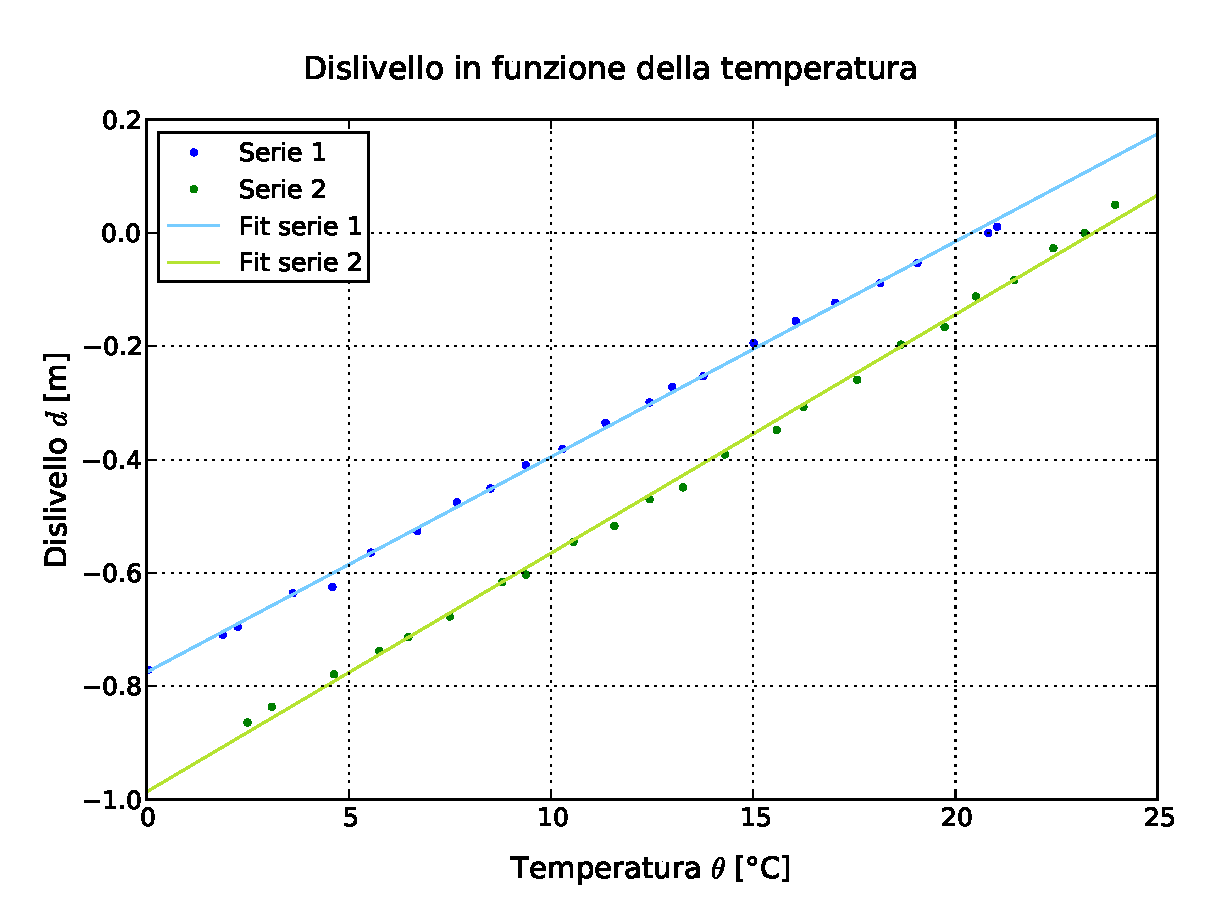
\includegraphics[width=110mm]{immagini/dislivello_temperatura.pdf}
    \caption{Il seguente grafico rappresenta}
    \label{fig:dislivello_temperatura}
\end{SCfigure}
%
Quindi in base a questi dati noi vogliamo verificare che la legge di prporzionalità diretta che lega la temperatura $\theta$ con il dislivello $d$ della colonnina di acqua sia corretta. Pertanto la legge si presenta come segue:

\begin{equation}
	h \,=\, A + B\,\theta
	\label{h_theta}
\end{equation}
%

    \subsubsection{Test del chi quadro}
\label{chi_1}

Sfruttiamo ora il test del $\chi^2$ per verificare se la regressione è corretta e se le incertezze sono accettabili.
In questo esperimento il $\chi^2$ è fondamentale, poiché le incertezze sui dati sono molto basse, e non molto realistiche;
correggendole speriamo di ottenere delle incertezze credibili che poi possano essere utilizzate per i calcoli successivi.

Non ci fidiamo molto delle incertezze calcolate nel paragrafo \ref{dati_incertezze}, poiché tengono conto solo degli errori
di risoluzione. Durante l'esperimento abbiamo notato che, soprattutto alle temperature più basse, la temperatura dell'acqua
variava (di qualche centesimo o anche decimo di grado) a seconda di dove era posizionata la sonda nel contenitore. Specialmente
al di sotto dei 4 gradi (quando la densità dell'acqua ricomincia a diminuire) abbiamo notato stratificazioni, con strati di acqua
più calda sul fondo del contenitore e più fredda in superficie, che faticavano a mescolarsi. Inoltre le temperature misurate
si riferiscono all'acqua e non all'aria contenuta nel vaso immerso, che non avevamo modo di misurare direttamente,
e non tengono conto delle possibili differenze di temperatura dell'aria all'interno del recipiente.
C'è quindi un errore sistematico dovuto alla difficoltà di definire le grandezze ``temperatura dell'acqua'' e ``temperatura dell'aria''
nonché nelle misure indirette della temperatura. 

Per tutti questi motivi sappiamo che
l'incertezza sulla temperatura è sicuramente sottostimata e va corretta. L'incertezza sulla lunghezza dovrebbe invece
essere più significativa, anche se non escludiamo che possa essere sottostimata anche quest'ultima. Tuttavia
al fine di semplificare i calcoli, da qui in avanti la
considereremo corretta e lavoreremo esclusivamente sulla temperatura.

Ci aspettiamo quindi che il valore del chi quadro sia molto alto e che non sia compatibile con il suo valore teorico. Il valore teorico
$\nu \equiv \chi\ped{teo}^2$ (utilizziamo $\nu$ per alleggerire la notazione) è uguale al numero di gradi di libertà meno
il numero di parametri calcolati con la regressione ed è diverso per le due serie di dati. Inoltre l'incertezza sul
$\nu$ vale $\delta \nu \equiv \delta \chi\ped{teo}^2 = \sqrt{2\nu}$. I due valori teorici sono quindi:

\begin{equation}
    \begin{array}{l @{\hspace{0.8cm}} c}
        \text{Serie 1:} & \nu_1 \pm \delta \nu_1 = 20 \pm 6 \\[3mm]
        \text{Serie 2:} & \nu_2 \pm \delta \nu_2 = 21 \pm 6
    \end{array}
\end{equation}
%
Premettiamo anche che adottiamo un fattore di copertura $k = 3$.
Per ciascuna serie, il chi quadro si calcola con la formula:

\begin{equation}
    \chi^2 \equiv \chi\ped{oss}^2 = \sum_{i=1}^{N} \frac{(d_i - A - B\theta_i)^2}{(\delta d\ped{tot})^2}
    \label{eq:chi2}
\end{equation}
%
dove $N$ è il numero di dati nella rispettiva serie. 

I risultati dei calcoli sono:

\begin{equation}
    \chi_1^2 = 9552 \qquad \qquad \chi_2^2 = 20741
\end{equation}
%
\`E evidente che, come ci aspettavamo, entrambi i $\chi^2$ delle due regressioni hanno valori molto alti, chiaramente non compatibili con
i valori teorici. Questo indica quantomeno una sottostima delle incertezze. In Figura \ref{fig:fit1} e \ref{fig:fit2} sono
graficate le discrepanza tra dati e rette di fit con le barre di incertezza, che come si vede sono molto piccole. Risulta ovvio il motivo del
valore così alto del $\chi^2$.

Tuttavia si possono vedere anche degli andamenti residui nei dati. Questo indica che non sono le incertezze l'unica
causa del fallimento del test del chi quadro, ma che probabilmente ci sono dei processi non considerati (errori sistematici)
che influenzano la dipendenza del dislivello dalla temperatura.

Non ci resta che aggiustare le incertezze per verificare se le correzioni da apportare sono realistiche; in caso affermativo
prenderemo come valide le incertezze corrette, altrimenti dovremo ``gettare a mare'' i risultati dei fit e studiare gli
andamenti residui.
Consideriamo accettabile un incertezza di circa 0.10 - 0.15 \si{\celsius}, poiché abbiamo verificato che la temperatura dell'acqua
variava, da una parte all'altra del contenitore, in questo ordine di grandezza. Un incertezza maggiore ci sembra improbabile.
L'aggiustamento va eseguito sulle due serie di dati separatamente.

Per aggiustare l'incertezza sulla temperatura, poiché è identica su tutte le misure, basta imporre:

\begin{equation}
    \nu = \sum_{i=1}^{N} \frac{(d_i - A - B\theta_i)^2}{(\delta d\ped{corr})^2}
\end{equation}
%
Da cui si può ricavare

\begin{equation}
    \delta d\ped{corr} = \sqrt{\sum_{i=1}^{N} \frac{(d_i - A - B\theta_i)^2}{\nu}}
    \label{eq:corr_err}
\end{equation}
%
Questa formula ci permette di calcolare l'incertezza sul dislivello che occorrerebbe avere affinché il valore del $\chi^2$
risulti uguale al suo valore teorico. Tuttavia, poiché crediamo che l'incertezza sottostimata sia quella sulla temperatura,
dobbiamo calcolare l'errore sulla temperatura corrispondente. Invertiamo quindi la formula (\ref{eq:err_tras_1}):

\begin{equation}
    \delta \theta\ped{corr} = \frac{\sqrt{\delta d\ped{corr}^2 - \delta d^2}}{B}
    \label{eq:corr_err_theta}
\end{equation}
%
dove B è il valore di pendenza ricavato dalla regressione e riferito alla serie di dati di cui stiamo correggendo l'incertezza.

I risultati dell'aggiustamento sono i seguenti (sono riportate le incertezze corrette sul dislivello per completezza):

\begin{equation}
    \delta d\ped{corr,1} = \SI{0.9}{\centi\meter} \qquad \qquad \delta d\ped{corr,2} = \SI{1.3}{\centi\metre}
\end{equation}
\begin{equation}
    \delta \theta\ped{corr,1} = \SI{0.24}{\celsius} \qquad \qquad \delta \theta\ped{corr,2} = \SI{0.32}{\celsius}
\end{equation}
%
I valori ottenuti sono abbastanza elevati. Come premesso, consideriamo realistico un errore di 0.10-0.15 \si{\celsius}.
Le incertezze corrette sono circa doppie e quindi ci sembrano troppo elevate per essere realistiche. In nessuna fase
dell'esperimento abbiamo notato una differenza così cospicua di temperatura all'interno del recipiente, ne crediamo che
il volume d'aria non termalizzato possa portare ad un incertezza di questo ordine di grandezza, in quanto molto minore
del volume di gas realmente termalizzato.

\begin{figure}[p]
    \centering
    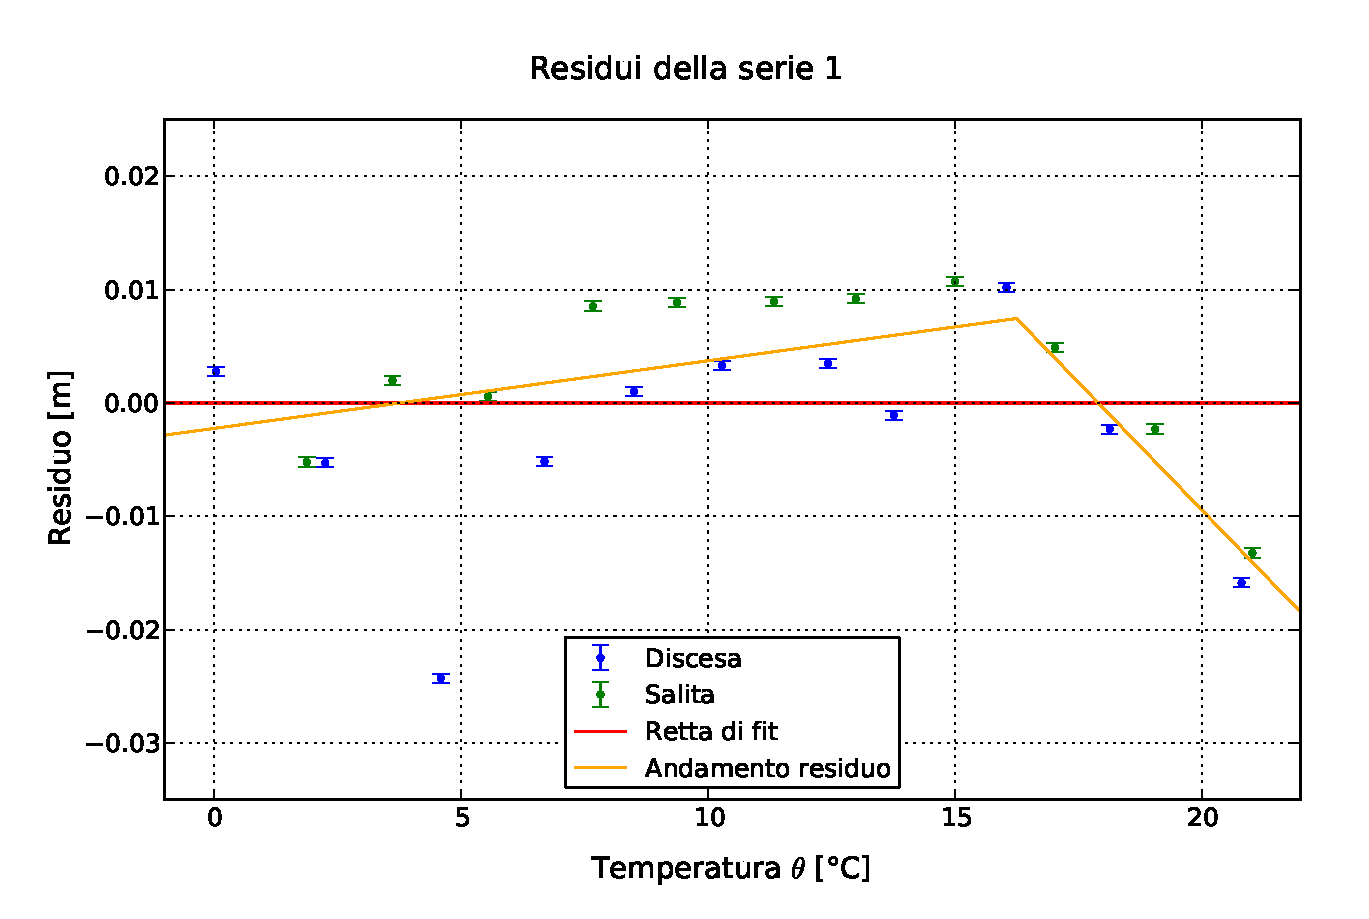
\includegraphics[width=118mm]{immagini/fit1.pdf}
    \caption{Il grafico in figura mostra i residui del fit sulla prima serie di dati. Sono riportati in colori
    diversi i dati presi abbassando (discesa) la temperatura e alzandola (salita). È evidente un andamento residuo nei dati,
    indicato approssimativamente in figura, probabilmente dovuto alla condensazione del vapor acqueo nella bottiglia. L'andamento
    residuo è formato da due rette che si incontrano attorno ai \SI{15}{\celsius}. L'ipotesi è che l'andamento residuo sia dovuto alla
    formazione di condensa all'interno del vaso, che rimuovendo molecole di gas dal recipiente, ha fatto abbassare la pressione e modificato
    la proporzionalità tra dislivello (pressione) e temperatura. C'è anche
    un dato con un residuo molto alto, visibile a sinistra della legenda.}
    \label{fig:fit1}
\end{figure}

\begin{figure}[p]
    \centering
    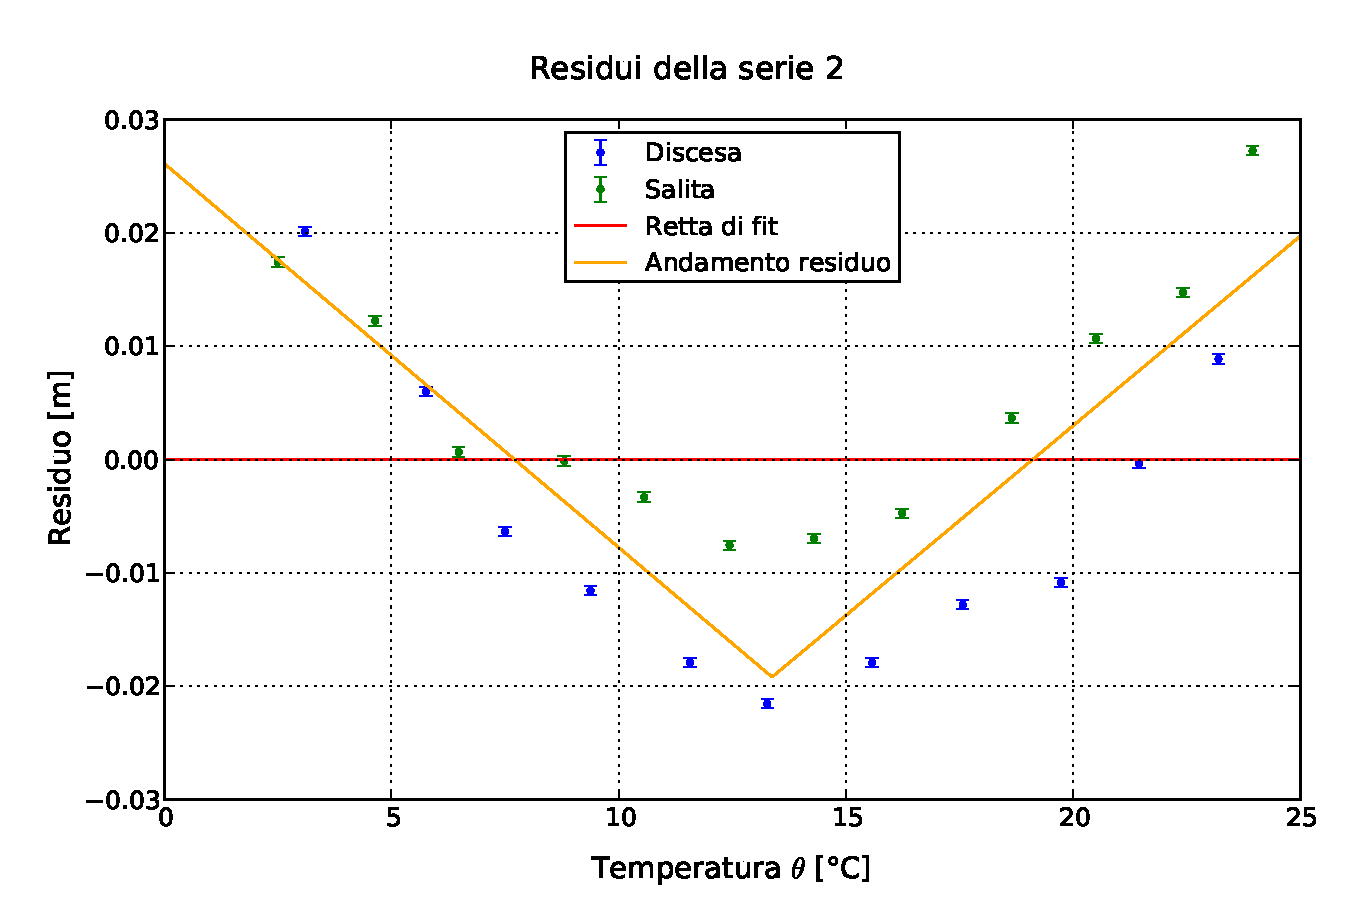
\includegraphics[width=117mm]{immagini/fit2.pdf}
    \caption{Sono riportati, rispettivamente in blu ed in verde, i residui dei dati ottenuti diminuendo ed aumentando la temperatura.
    La retta spezzata indica approssimativamente l'andamento residuo osservato, anche se sarebbe possibile distinguere due residui
    diversi durante salita e discesa. Si vede infatti che i punti misurati salendo hanno un dislivello minore, a parità di temperatura
    rispetto agli altri, il che significa che la pressione interna era maggiore. Un modo di spiegare questa anomalia è l'ipotesi che
    alle temperature basse, quando il vaso era a pressione minore di quella atmosferica, ci sia stata una perdita e dell'aria sia entrata
    nel recipiente, aumentando quindi le moli di aria e la relazione tra temperatura e dislivello (pressione).}
    \label{fig:fit2}
\end{figure}

Riteniamo quindi che l'errore vada cercato altrove. In Figura \ref{fig:fit1} e \ref{fig:fit2} sono riportati i residui delle due
serie di dati. Si notano degli andamenti residui, disegnati nei grafici, che assumono approssimativamente la forma di linea spezzata.
Ci sono stati quindi dei processi, durante l'esecuzione dell'esperimento, che non abbiamo preso in considerazione.
Questi errori sistematici spiegno come mai il $\chi^2$ è così alto e perché le incertezze corrette non sono verosimili. I parametri calcolati con
le regressioni precedenti sono privi di senso e anche le rette di fit in realtà sono prive di significato, poiché non
descrivono completamente il fenomeno osservato.

    \subsubsection{Cause degli andamenti residui}

Nel paragrafo precedenti si sono riscontrati degli evidenti andamenti residui. Come conseguenza la legge lineare ottenuta
si adatta male ai dati, il $\chi^2$ è molto alto, come alte sono le correzioni da apportare alle incertezze affinché 
il valore del chi quadro risulti corretto. Certo, l'incertezza stimata inizialmente, che tiene conto solo degli errori di risoluzione
è sicuramente sottostimata e va corretta, ma portare l'incertezza sulla temperatura sino a \SI{0.3}{\celsius} non è accettabile.
Inoltre gli andamenti residui indicano che ci sono stati dei processi di cui non si è tenuto conto durante l'esecuzione dell'esperimento.

Ma quali sono i processi che hanno provocato tali andamenti? Dobbiamo fare qualche ipotesi e constatazione. Innanzitutto,
facciamo notare che gli andamenti residui per le due serie di dati sono di diversa natura. Le figure \ref{fig:fit1} e
\ref{fig:fit2} mostrano residui opposti rispetto alle rette calcolate nel paragrafo \ref{reg_1}. Nel caso della prima
serie di dati (figura \ref{fig:fit1}), la pendenza dell'andamento residuo è minore a quella della retta di fit a
temperature alte e maggiore a temperature basse, mentre nel caso della seconda serie di dati (figura \ref{fig:fit2}) è
vero il contrario.

In secondo luogo, i residui sono ben rappresentati da rette spezzate, seppur con qualche imprecisione.

Nel caso della prima serie di dati, l'ipotesi che ci sembra spiegare meglio l'andamento residuo osservato è la condenazione
del vapor acqueo, che era presente all'interno del vaso. Probabilmente attorno ai \SI{15}{\celsius}, punto in cui la linea
è spezzata, il vapore acqueo ha iniziato a condensare, togliendo molecole al gas e cambiando la correlazione tra dislivello e
temperatura. Secondo questa ipotesi la pressione (dislivello) a temperature più basse dovrebbe essere minore di quella prevista
con il residuo dei dati a temperature alte, che è quello che il grafico suggerisce.
Affinché questa ipotesi risulti valida occorre anche ipotizzare che la condensazione abbia proceduto ad un ritmo circa costante,
poiché la retta dovrebbe diventare meno pendente in presenza di meno gas, mentre quello che si osserva è che la pendenza aumenta.
Ipotizzando che la condensazione (e chiaramente anche l'evaporazione durante la salita) sia stata costante si può spiegare 
l'andamento residuo. 

\subsubsection{Regressione residui}

Poiché gli andamenti residui sono ben rappresentati da rette spezzate, abbiamo pensato di ovviare a tutti questi problemi suddividendo i
dati in vari gruppi in base agli andamenti residui, in modo da poter eseguire la regressione lineare per ogni gruppo di dati.
Abbiamo fatto quanto segue:

\label{sottoserie}
\begin{itemize}
    \item{Innanzitutto abbiamo eliminato un dato nella prima serie di misure, in quanto era probabilmente il frutto di un
        errore di misura. Questo dato, visibile in figura \ref{fig:fit1} a fianco della legenda,
        contribuiva molto al valore del $\chi^2$, ed era completamente scollegato dal resto della serie.}
    \item{Dalla prima serie di misure sono stati estratti due gruppi di dati, il primo formato da tutte le misure fatte
        a temperatura superiore a \SI{15}{\celsius} e il secondo da tutte quelle fatte a temperatura inferiore, eccetto
        il dato che è stato tolto.}
    \item{Dalla seconda serie, abbiamo estratto altri due gruppi di dati, uno con i dati rilevati a temperature maggiori di
        \SI{14}{\celsius}, e l'altro con i dati rimanenti.}
\end{itemize}

La Tabella \ref{tab:gruppi}, estratta dalla Tabella \ref{tab:dati} riporta i vari gruppi in cui sono stati suddivisi i dati.

\begin{SCtable}{}{b}
    \centering
    \begin{tabular}{l  c c @{\hspace{0.8cm}} c c @{\hspace{0.8cm}} c c @{\hspace{0.8cm}} c c}
        \multicolumn{9}{c}{\textbf{Gruppi di dati}} \\
        \toprule
        & $\theta$ & $d$ & $\theta$ & $d$ & $\theta$ & $d$ & $\theta$ & $d$ \\ 
        \midrule
        & 20.81 &  0.000 & 13.77 & -0.253 & 23.20 &  0.000 & 13.27 & -0.449 \\
        & 18.14 & -0.088 & 12.44 & -0.299 & 21.45 & -0.083 & 11.57 & -0.517 \\
        & 16.05 & -0.155 & 10.29 & -0.381 & 19.73 & -0.166 &  9.38 & -0.603 \\
        & 15.01 & -0.194 &  8.51 & -0.451 & 17.57 & -0.259 &  7.50 & -0.677 \\
        & 17.03 & -0.123 &  6.70 & -0.526 & 15.58 & -0.348 &  5.76 & -0.738 \\
        & 19.06 & -0.053 &  2.26 & -0.695 & 14.30 & -0.391 &  3.10 & -0.836 \\
        & 21.03 &  0.011 &  0.05 & -0.771 & 16.24 & -0.307 &  2.50 & -0.864  \\
        &       &        &  1.89 & -0.709 & 18.65 & -0.197 &  4.64 & -0.779 \\
        &       &        &  3.62 & -0.636 & 20.50 & -0.112 &  6.48 & -0.713 \\
        &       &        &  5.55 & -0.564 & 22.42 & -0.027 &  8.80 & -0.616 \\
        &       &        &  7.68 & -0.475 & 23.95 &  0.050 & 10.56 & -0.545 \\
        &       &        &  9.38 & -0.410 &       &        & 12.44 & -0.470 \\
        &       &        & 11.35 & -0.335 &       &        &       &        \\
        &       &        & 13.00 & -0.272 &       &        &       &        \\
        \midrule
        $N_j$ & \multicolumn{2}{c}{7} &  \multicolumn{2}{c}{14} & \multicolumn{2}{c}{11} & \multicolumn{2}{c}{12} \\
        \bottomrule
    \end{tabular}
    \caption{}
    \label{tab:gruppi}
\end{SCtable}

Dopo aver suddiviso i dati in questo modo abbiamo calcolato la retta di fit per ogni gruppo di dati, in modo da ottenere
4 rette. Come nei paragrafi precedenti abbiamo seguito la seguenti procedura:

\begin{itemize}
    \item{Per ogni set di dati $j$-esimo è stato eseguito un fit preliminare sui dati,
            minimizzando la seguente funzione (metodo dei minimi quadrati)
            \begin{equation}
                \sum_{i=1}^{N_j} \frac{(d - A_j' - B_j'\theta)^2}{\delta d}
            \end{equation}
            dove $N_j$ indica il numero di dati nel gruppo $j$-esimo, $A_j'$ e $B_j'$ sono rispettivamente
            le stime dell'intercetta e del coefficiente angolare della retta di fit, sempre per il gruppo $j$-esimo.
            Per la stima preliminare si è usata soltanto l'incertezza $\delta d$.
        }
\end{itemize}

I risultati del fit preliminare ed i risultati della regressione finale sono riportati nella seguente tabella.

\begin{center}
    \begin{tabular}{c c | c c c c}
        \toprule
        \multicolumn{2}{c|}{Fit preliminare} & \multicolumn{4}{c}{Regressione finale} \\
        \midrule
        $B'$ & $\delta B'$ & A & $\delta A$ & B & $\delta B$ \\
        $[\si{\centi\meter\per\celsius}]$ & $[\si{\centi\meter\per\celsius}]$ &
        [m] & [m] & $[\si{\centi\meter\per\celsius}]$ & [\si{\centi\metre\per\celsius}] \\
        \midrule
        3.353 & 0.007 & -0.695  & 0.001 & 3.353 & 0.007 \\
        3.890 & 0.003 & -0.7815 & 0.0002 & 3.890 & 0.003 \\
        4.550 & 0.004 & -1.0508 & 0.0008 & 4.550 & 0.004 \\
        3.877 & 0.003 & -0.9607 & 0.0003 & 3.877 & 0.004 \\
        \bottomrule
    \end{tabular}
\end{center}

È evidente la compatibilità di tutti i valori $B'$, ottenuti dalle regressioni preliminari, con i rispettivi valori $B$ ottenuti dai
fit finali. I valori di $B'$ e $B$ sono infatti uguali entro l'incertezza in tutti e 4 i casi.

    \subsubsection{Chi quadro residui}

Come prima, usiamo nuovamente il test del $\chi^2$ per valutare le incertezze. Come già ripetuto più volte,
le incertezze sono sottostimate e quindi vogliamo fare il test del chi quadro, il cui risultato non sarà compatibile con il valor atteso,
e poi lo useremo per aggiustare gli errori.

I valori attesi $\nu \equiv \chi\ped{teo}^2$, per ciascuna sottoserie di dati, sono uguali al numero di gradi di libertà,
ovvero al numero di dati $N_j$ del gruppo $j$-esimo meno due, che è il numero di parametri calcolati con la regressione.
L'incertezza $\delta \nu$ si calcola con la formula $\delta \nu = \sqrt{2\nu}$. Inoltre prendiamo un fattore di copertura
$k = 3$.

Dopodiché è stato calcolato il $\chi^2$ con la formula (\ref{eq:chi2}) del paragrafo \ref{chi_1}.

La seguente tabella riporta i valori attesi per ogni gruppo, con relative incertezze ed anche i corrispondenti valori del chi quadro.

\begin{center}
    \begin{tabular}{l c c c c}
        \multicolumn{5}{c}{\textbf{Valori teorici del $\chi^2$}} \\
        \toprule
        & Gruppo 1 & Gruppo 2 & Gruppo 3 & Gruppo 4 \\
        \midrule
        $N_j$ & 7 & 14 & 11 & 12 \\
        $\nu$ & 5 & 12 & 9 & 10 \\
        $\delta \nu$ & 3 & 5 & 4 & 4 \\
        $\chi^2$ & 159 & 1521 & 3587 & 1541 \\
        \bottomrule
    \end{tabular}
\end{center}

Osserviamo immediatamente che nessuno dei valori del chi quadro è compatibile con il suo valore teorico entro l'intervallo di confidenza.
Come atteso, è necessario aggiustare le incertezze, tuttavia i valori del $\chi^2$ sono significativamente più bassi rispetto a
quelli ottenuti prima di dividere i dati in sottoserie.

L'aggiustamento delle incertezze si svolge come già spiegato nel paragrafo \ref{chi_1} con la formula (\ref{eq:corr_err}).
Il calcolo dell'incertezza sulla temperatura si svolge come indicato nella formula (\ref{eq:corr_err_theta}).
Svolgendo la procedura si ottengono le seguenti incertezze corrette sulla temperatura.

\begin{center}
    \begin{tabular}{l c c c c}
        \multicolumn{5}{c}{\textbf{Incertezze corrette sulla temperatura}} \\
        \toprule
        & Gruppo 1 & Gruppo 2 & Gruppo 3 & Gruppo 4 \\
        \midrule
        $\delta d\ped{corr}$ [cm] & 0.2 & 0.5 & 0.9 & 0.5 \\
        $\delta \theta\ped{corr}$ [\si{\celsius}] & 0.07 & 0.12 & 0.19 & 0.14 \\
        \bottomrule
    \end{tabular}
\end{center}

Ora queste incertezze ci sembrano molto più realistiche di quelle ricavate in precedenza, infatti, a parte l'incertezza del 
gruppo 3, sono tutte attorno a \SI{0.10}{\celsius}. Notiamo anche che l'errore sui gruppi 3 e 4 sono più alti, come era possibile aspettarsi.
Nella seconda serie di dati c'è infatti un errore sistematico per il quale le pressioni in salita sono minori di quelle in discesa.

Nonostante la presenza di questo errore, abbiamo deciso di accettare le incertezze che abbiamo qui calcolato, in quanto
sono sicuramente migliori delle incertezze di risoluzione accettate in origine.

Dopo aver corretto le incertezze occorre eseguire nuovamente i fit sui gruppi di dati, per ottenere le nuove incertezze sui parametri
$A$ e $B$. Eseguendo nuovamente il metodo dei minimi quadrati con le nuove incertezze si ottengono i seguenti dati.

\begin{center}
    \begin{tabular}{l c c c c}
        \multicolumn{5}{c}{\textbf{Incertezze corrette su $A$ e $B$}} \\
        \toprule
        & Gruppo 1 & Gruppo 2 & Gruppo 3 & Gruppo 4 \\
        \midrule
        $\delta A$ [cm] & 0.77 & 0.26 & 1.65 & 0.39 \\
        $\delta B$ [\si{\centi\metre\per\celsius}] & 0.04 & 0.03 & 0.08 & 0.04 \\
        \bottomrule
    \end{tabular}
\end{center}

\begin{SCfigure}[][!b]
    \centering
    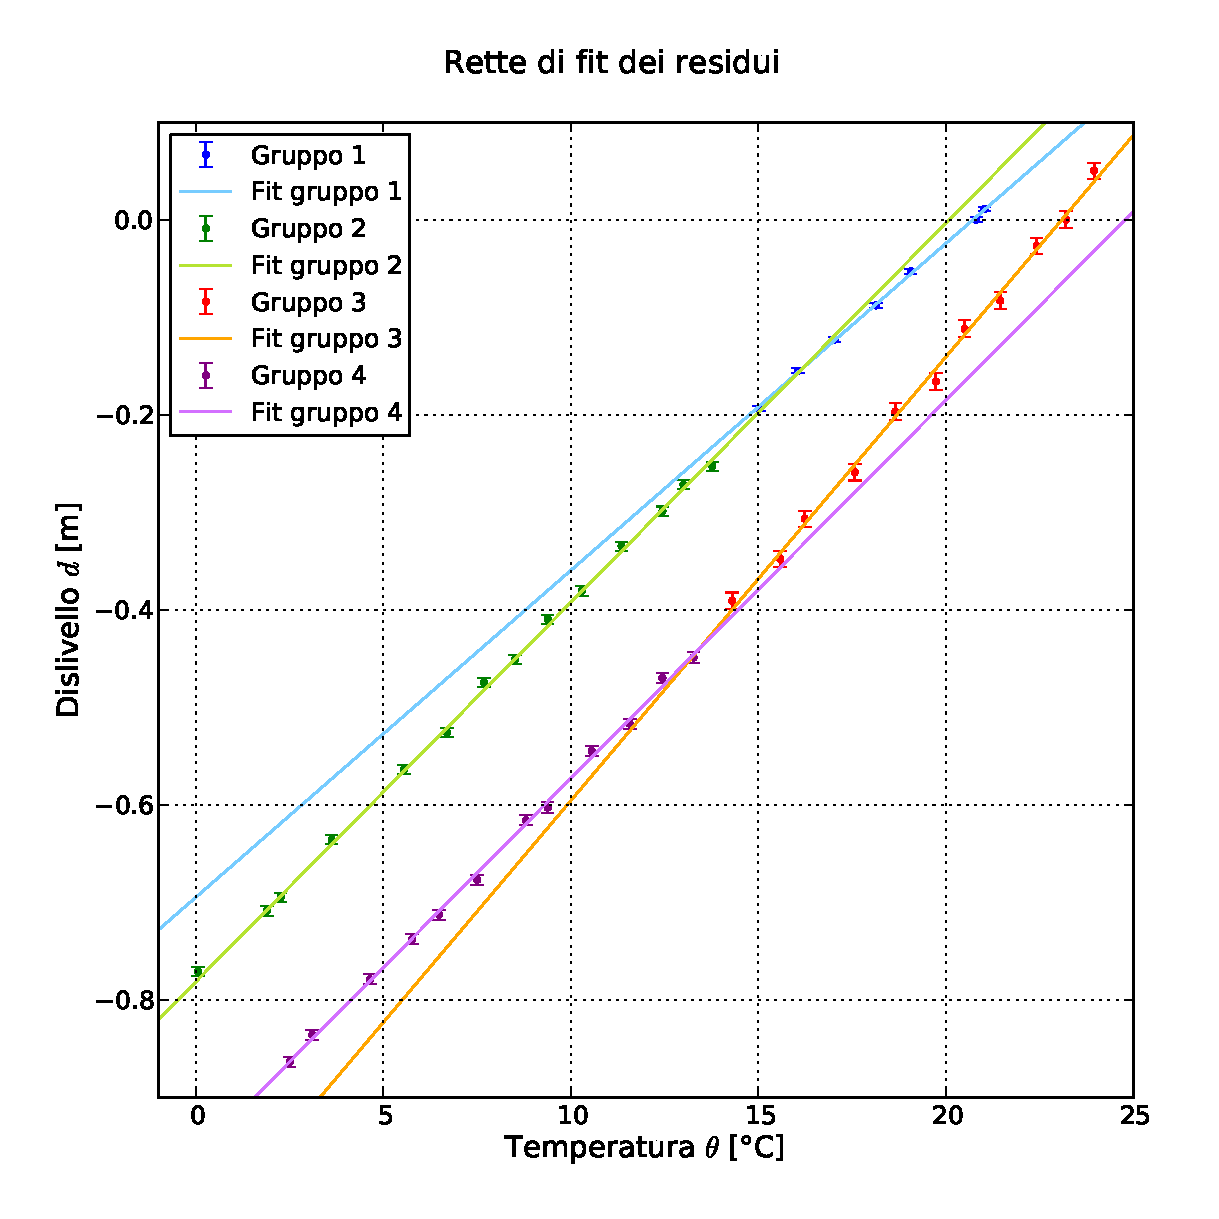
\includegraphics[width=120mm]{immagini/residui.pdf}
    \caption{Il grafico riporta visivamente le quattro regressioni eseguite sui gruppi di dati.
    Le rette si adattano ai dati in maniera sensibilmente migliore di quanto non succedesse prima
    di creare le sottoserie. Le incertezze riportate sono gli errori sul dislivello corretti, diversi
    da gruppo a gruppo. }
    \label{fig:residui}
\end{SCfigure}

\begin{figure}[p]
    \centering
    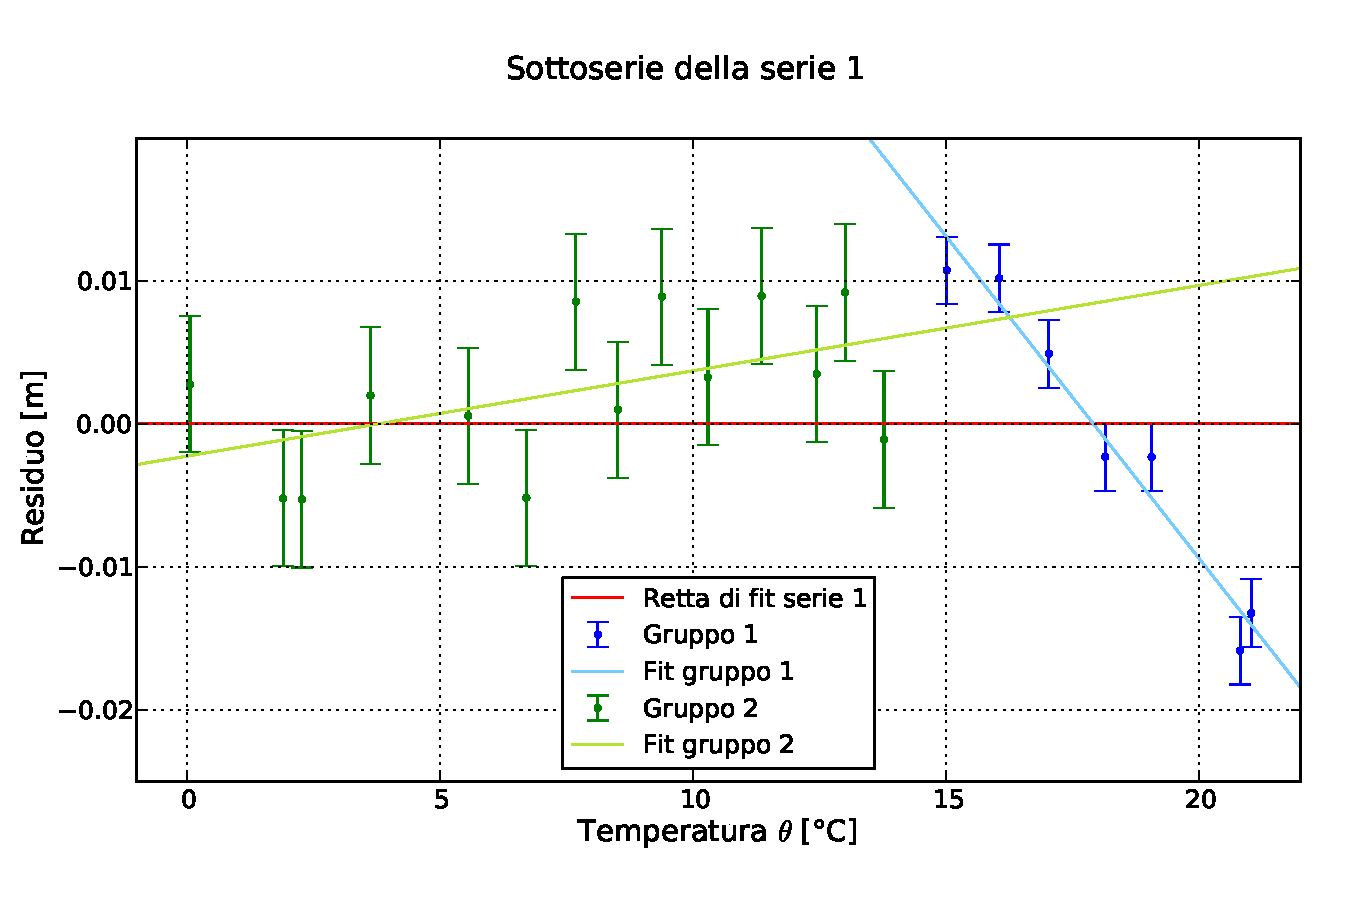
\includegraphics[width=130mm]{immagini/fit1r.pdf}
    \caption{Dettaglio dei residui della prima serie. Il grafico è analogo a quello in figura \ref{fig:fit1},
    solo che qui sono evidenziati i gruppi 1 e 2, ricavati dalla prima serie, che sono
    riportati con colori ed incertezze diverse. I colori sono uguali a quelli della Figura \ref{fig:residui},
    per facilitare il confronto, mentre le incertezze riportate sono le incertezze corrette sul dislivello.}
    \label{fig:fit1r}
\end{figure}

\begin{figure}[p]
    \centering
    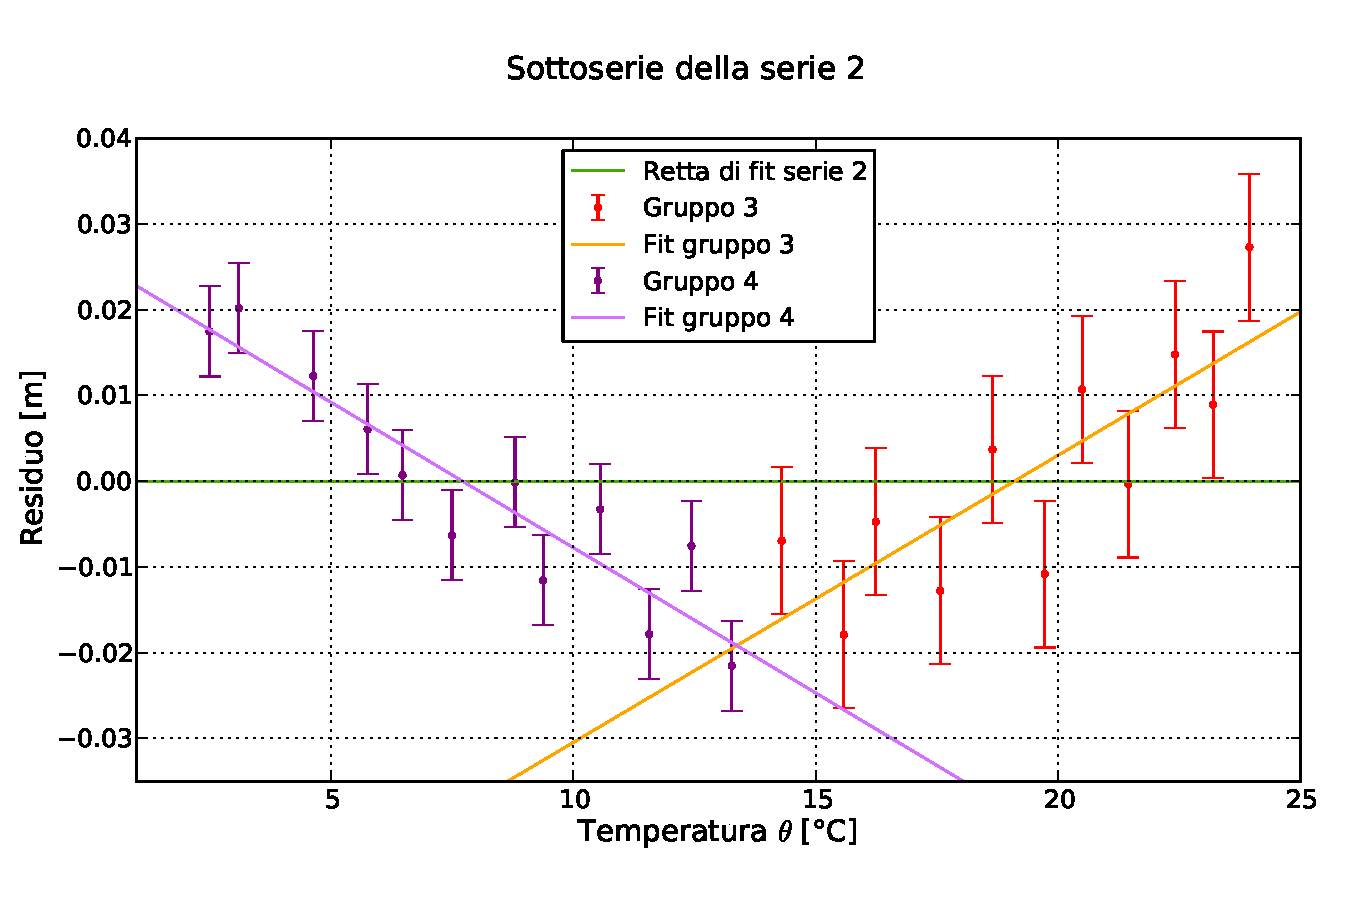
\includegraphics[width=130mm]{immagini/fit2r.pdf}
    \caption{Analogamente all'immagine precedente, questo plot è simile a quello in Figura \ref{fig:fit2},
    tranne che sono graficati distintamente i punti dei gruppi 3 e 4. Le incertezze riportate sono le incertezze
    corrette sul dislivello.}
    \label{fig:fit2r}
\end{figure}

\newpage
\section{Calcolo dello zero assoluto}

Una volta ricavati gli andamenti lineari di $d$ in funzione di $\theta$, proseguiamo nel determinare il valore dello zero assoluto.
Data la pressione atmosferica $P_A$, e presi $g = \SI{9.807}{\meter\per\square\second}$ e
$\rho = \SI{1000}{\kilo\gram\per\cubic\metre}$ parametri di cui ignoriamo l'incertezza, sappiamo che:

\begin{equation}
	P \,\, = \,\, P_A + \rho g d \,\, = \,\, P_A + \rho g (A + B \theta) \,\, = \,\, f(\theta)
\end{equation}
%
che pone in relazione la pressione del gas con la temperatura da noi calcolata. Lo zero assoluto è la temperatura a cui la
pressione $P$ esercitata dal gas va a zero. Invertendo l'equazione sopra e ponendo $P = 0$ si ottiene:

\begin{equation}
	\theta_0 \,\, = \,\, - \frac{1}{B} \left( \frac{P_A}{pg} + A \right)
    \label{eq:t0}
\end{equation}
%
Utilizzando le regole di propagazione dell'incertezza si ottiene:

\begin{equation}
    \delta \theta_0 \,\, = \,\, \sqrt{\left(\frac{1}{B \rho g}\right)^2 (\delta P_A)^2 +
    \left(\frac{1}{B}\right)^2 (\delta A)^2 + \left(\frac{P_A + \rho g A}{B^2 \rho g} \right)^2 \delta B^2}
    \label{eq:dt0}
\end{equation}


\subsection{Utilizzo dei dati di pressione}
\label{press}

Nelle formule (\ref{eq:t0}) e (\ref{eq:dt0}) si sono usati i valori $P_A$ e $\delta P_A$ che finora non sono stati calcolati.
Essi indicano il valore della pressione atmosferica durante l'esperimento. La Tabella \ref{tab:ptu} riporta i valori di pressione atmosferica
$P_{A,i}$ rilevati durante l'esperimento. Poiché per ogni giorno sono stati presi 15 valori (cioè $i \in \{1, \dots, 15\}$)
di pressione, lo scopo di questo paragrafo è ricavare due valori, con relativa incertezza, della pressione atmosferica nelle
due giornate. Abbiamo infatti deciso di ottenere un unica media per ogni giornata in quanto durante le due giornate il tempo metereologico e la
pressione atmosferica sono rimasti approssimativamente costanti e nella (\ref{eq:t0}) possiamo usare un solo valore $P_A$.

I calcoli che seguono sono stati eseguiti due volte per i dati delle due giornate.
Come valore di $P_A$ si è presa la media aritmetica delle pressioni atmosferiche $P_{A,i}$ rilevate:

\begin{equation}
    P_A = m^*(P_{A,i}) = \frac{1}{N}\sum_{i=1}^N P_{A,i}
\end{equation}
%
dove $N = 15$ è il numero di misure fatte. Mentre come stimatore della varianza abbiamo usato la deviazione standard sulla media.
Non è stato preso in considerazione l'errore di risoluzione in quanto esso è trascurabile rispetto all'errore statistico. 

\begin{equation}
    \delta P_A = \sigma^*(P_{A}) = \sqrt{\frac{1}{N(N-1)}\sum_{i=1}^N (P_{A,i} - P_A)^2}
\end{equation}
%
Otteniamo quindi due misure relative alle due serie:

\begin{equation}
    P_{A1} \pm \delta P_{A1} = (96237 \pm 47) \; \si{\pascal} \qquad P_{A2} \pm P_{A2} = (97302 \pm 72) \; \si{\pascal}
    \label{eq:pa}
\end{equation}
%
dove le cifre significative sono state arrotondate all'ordine di grandezza dall'incertezza.

%\subsection{Confronto dei dati delle serie con il valore noto}
%\label{confronto}
%Prima di verificare la compatibilià tra il valore noto e i valori di $\theta_0$ delle due serie di dati, poniamo un fattore di copertura $k=3$. Sapendo che il valore noto è -273.15, il procedimento per verificare la compatibilià si compone di:
%
%\begin{itemize}
%\item Calcolare la discrepanza $R$ tra $\theta_{0,i}$ e il valore noto:
%\begin{equation*}
%	R \,\, = \,\, \theta_{0,i} - (-273.15)
%\end{equation*}
%\item controllare se:
%\begin{equation*}
%	R \,\, \leq \,\, k \sigma[\theta_{0,i}]
%\end{equation*}
%\end{itemize}
%
%Eseguendo tale procedura su i valori di ognuna delle due serie, si ottiene che entrambi i valori $\theta_{0,1}$ e $\theta_{0,2}$ non risultano essere compatibili con il valore noto.
%
%Ciò è probabilmente dovuto al fatto che il modello teorico non tiene in considerazione importanti fattori come la diversa termalizzazione del gas o la presenza di vapore nel gas che possono provocare anche consistenti errori sistematici.
%\bigskip
%
%Per questo motivo abbiamo spezzato i dati ricavati in diverse sottoserie per ottenere dei fit migliori ed evidenziare gli errori sistematici.

\subsection{Calcolo dello zero dalle regressioni}

Nel paragrafo {\ref{sottoserie}} abbiamo ottenuto quattro diverse rette di fit. Per ciascuna retta abbiamo calcolato
il rispettivo zero assoluto grazie alle formule (\ref{eq:t0}) e (\ref{eq:dt0}) e ai valori di pressione (\ref{eq:pa}). Si ottengono i seguenti
valori:

\begin{center}
    \begin{tabular}{l c c c c}
        \multicolumn{5}{c}{\textbf{Zero assoluto}} \\
        \toprule
        & Gruppo 1 & Gruppo 2 & Gruppo 3 & Gruppo 4 \\
        \midrule
        $\theta_0$ [\si{\celsius}] & -272 & -234 & -195 & -231 \\
        $\delta \theta_0$ [\si{\celsius}] & 3 & 3 & 4 & 3 \\
        \bottomrule
    \end{tabular}
\end{center}

La tabella mostra i valori dello zero assoluto calcolati partendo dalle regressioni sulle quattro sottoserie di dati.
I dati sono riportati con precisione data dall'incertezza.
  
\subsection{Confronto dei dati delle sottoserie con il valore noto}

Commentiamo brevemente i risultati e la loro compatibilità
con il valore noto $T_0 = \SI{-273.15}{\celsius}$. Per la compatibilità adottiamo un fattore di copertura $k = 3$.

\begin{itemize}
    \item{\textbf{Gruppo 1.} Il valore ottenuto è molto vicino a quello teorico ed è compatibile con quello teorico
        a meno di un sigma.}

    \item{\textbf{Gruppo 2.} Il valore ottenuto non è compatibile con quello teorico, infatti
        
        \begin{equation}
            R = |T_0 - \theta_0| \simeq \SI{39}{\celsius} \qquad \text{e} \qquad k\delta \theta_0 = \SI{9}{\celsius} < R
        \end{equation}

        Se prendiamo per certo il valore teorico (verificato sperimentalmente da fisici sperimentali senza dubbio migliori
        di noi), questo è un ulteriore indizio che l'effetto residuo che ha scombinato i conti era presente solo nel gruppo 2.
        Questa è una conferma dell'ipotesi della condensazione dell'acqua, che prevede, correttamente, effetti solo sulla serie 2.
        Chiaramente non sono escluse altre ipotesi.}

    \item{\textbf{Gruppo 3.} Il valore calcolato è molto lontano e non compatibile (si confronti con il precedente) con il valore
        teorico. Sicuramente qui c'è qualche grosso errore nell'esecuzione dell'esperimento.}
    
    \item{\textbf{Gruppo 4.} In questo caso il discorso è analogo a quello fatto per il gruppo 2.}
\end{itemize}

Concludiamo dicendo che i valori sperimentali dello zero assoluto ottenuti non sono soddisfacenti in quanto tre su quattro
non sono compatibili con il valore teorico, ma soprattutto non sono nemmeno compatibili tra di loro. Il motivo è probabilmente che i dati raccolti con questo esperimento sono di scarsa qualità, poiché l'esperimento è stato affetto da errori sistematici.


\newpage
\section{Conclusioni}
In questo esperimento abbiamo utilizzato due diversi procedimenti meccanici per la misura di una stessa grandezza: la costante elastica della molla. I due procedimenti si differenziano per il diverso utilizzo della molla: il primo necessita di un uso statico (misurazione dell'elongazione), mentre il secondo di un uso dinamico (misurazione del periodo di oscillazione). Ogni procedimento ha portato all'ottenimento di un valore della costante elastica e, inoltre, ogni valore della costante è stato a sua volta ottenuto sia con procedure grafiche sia con procedure analitiche.
Seguire non una sola procedura, ma entrambe, ci ha permesso una maggiore sicurezza sulla validità del risultato ottenuto. Ogni procedura ha infatti funto da controprova per l'altra e, come mostrato nel precedente paragrafo, i coefficienti elastici ricavati con il metodo statico e con il metodo dinamico risultano compatibili, ponendo come fattore di copertura $k\,=\,3$.

In questo stesso esperimento ci interessava, inoltre, verificare la linearità della risposta della molla in funzione della forza ad essa applicata. Questo obiettivo è stato raggiunto e, come si può vedere dalle tabelle e dai grafici, la linearità è stata appurata in un adeguato range di valori.
È in aggiunta stato verificato che la molla non si deformasse in modo definitivo a causa dei pesi a cui era stata sottoposta, vanificando tutto l'esperimento.
\\
\\


\textbf{Disclaimer}: Nonostante i componenti del gruppo B11 ci vogliano affibbiare la colpa del fatto che il loro esperimento non è andato a buon fine, noi decliniamo apertamente ed a gran voce ogni responsabilità.

\end{document}
